\documentclass{article}
\usepackage{tikz}
\usetikzlibrary{calc,fadings,decorations.pathreplacing,shadings}
\usepackage{verbatim}

\newcommand\pgfmathsinandcos[3]{%
  \pgfmathsetmacro#1{sin(#3)}%
  \pgfmathsetmacro#2{cos(#3)}%
}
\newcommand\LongitudePlane[3][current plane]{%
  \pgfmathsinandcos\sinEl\cosEl{#2} % elevation
  \pgfmathsinandcos\sint\cost{#3} % azimuth
  \tikzset{#1/.style={cm={\cost,\sint*\sinEl,0,\cosEl,(0,0)}}}
}

\newcommand\LatitudePlane[3][current plane]{%
  \pgfmathsinandcos\sinEl\cosEl{#2} % elevation
  \pgfmathsinandcos\sint\cost{#3} % latitude
  \pgfmathsetmacro\yshift{\RadiusSphere*\cosEl*\sint}
  \tikzset{#1/.style={cm={\cost,0,0,\cost*\sinEl,(0,\yshift)}}} %
}
\newcommand\NewLatitudePlane[4][current plane]{%
  \pgfmathsinandcos\sinEl\cosEl{#3} % elevation
  \pgfmathsinandcos\sint\cost{#4} % latitude
  \pgfmathsetmacro\yshift{#2*\cosEl*\sint}
  \tikzset{#1/.style={cm={\cost,0,0,\cost*\sinEl,(0,\yshift)}}} %
}
\newcommand\DrawLongitudeCircle[2][1]{
  \LongitudePlane{\angEl}{#2}
  \tikzset{current plane/.prefix style={scale=#1}}
   % angle of "visibility"
  \pgfmathsetmacro\angVis{atan(sin(#2)*cos(\angEl)/sin(\angEl))} %
  \draw[current plane] (\angVis:1) arc (\angVis:\angVis+180:1);
  \draw[current plane,opacity=0.4] (\angVis-180:1) arc (\angVis-180:\angVis:1);
}
\newcommand\DrawLongitudeArc[4][black]{
  \LongitudePlane{\angEl}{#2}
  \tikzset{current plane/.prefix style={scale=1}}
  \pgfmathsetmacro\angVis{atan(sin(#2)*cos(\angEl)/sin(\angEl))} %
  \pgfmathsetmacro\angA{mod(max(\angVis,#3),360)} %
  \pgfmathsetmacro\angB{mod(min(\angVis+180,#4),360} %
  \draw[current plane,#1,opacity=0.4] (#3:\RadiusSphere) arc (#3:#4:\RadiusSphere);
  \draw[current plane,#1]  (\angA:\RadiusSphere) arc (\angA:\angB:\RadiusSphere);
}%
\newcommand\DrawLatitudeCircle[2][1]{
  \LatitudePlane{\angEl}{#2}
  \tikzset{current plane/.prefix style={scale=#1}}
  \pgfmathsetmacro\sinVis{sin(#2)/cos(#2)*sin(\angEl)/cos(\angEl)}
  % angle of "visibility"
  \pgfmathsetmacro\angVis{asin(min(1,max(\sinVis,-1)))}
  \draw[current plane] (\angVis:1) arc (\angVis:-\angVis-180:1);
  \draw[current plane,opacity=0.4] (180-\angVis:1) arc (180-\angVis:\angVis:1);
}

\newcommand\DrawLatitudeArc[4][black]{
  \LatitudePlane{\angEl}{#2}
  \tikzset{current plane/.prefix style={scale=1}}
  \pgfmathsetmacro\sinVis{sin(#2)/cos(#2)*sin(\angEl)/cos(\angEl)}
  % angle of "visibility"
  \pgfmathsetmacro\angVis{asin(min(1,max(\sinVis,-1)))}
  \pgfmathsetmacro\angA{max(min(\angVis,#3),-\angVis-180)} %
  \pgfmathsetmacro\angB{min(\angVis,#4)} %
  \draw[current plane,#1,opacity=0.4] (#3:\RadiusSphere) arc (#3:#4:\RadiusSphere);
  \draw[current plane,#1] (\angA:\RadiusSphere) arc (\angA:\angB:\RadiusSphere);
}


\newcommand{\AxisRotator}[1][rotate=0]{%
    \tikz [x=0.25cm,y=0.60cm,line width=.2ex,-stealth,#1] \draw (0,0) arc (-150:150:1 and 1);%
}
%% document-wide tikz options and styles

\tikzset{%
  >=latex, % option for nice arrows
  inner sep=0pt,%
  outer sep=2pt,%
  mark coordinate/.style={inner sep=0pt,outer sep=0pt,minimum size=3pt,
    fill=black,circle}%
}

\begin{document}

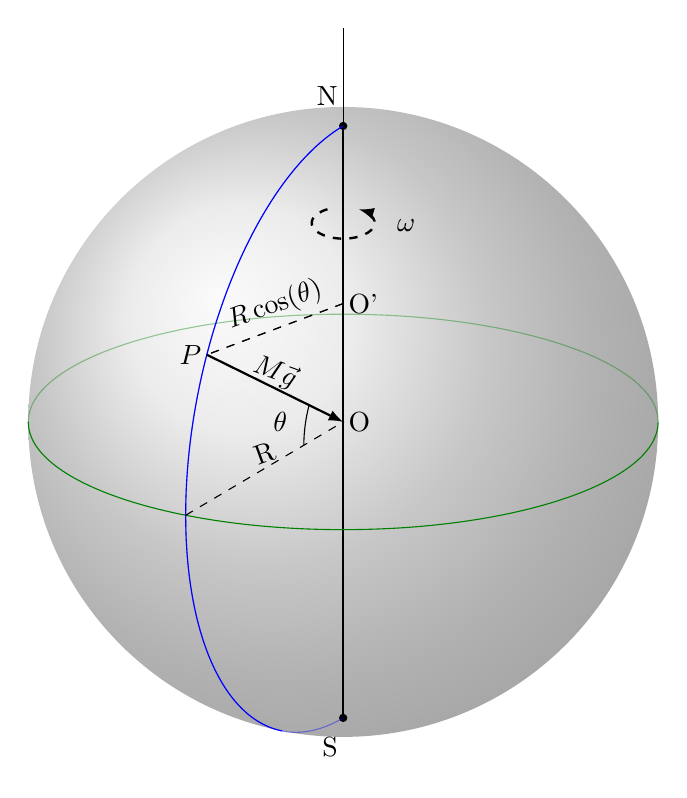
\begin{tikzpicture} % "THE GLOBE" showcase
\def\RadiusSphere{4} % sphere radius
\def\angEl{20} % elevation angle
\def\angAz{-20} % azimuth angle

\shade[ball color = gray!40, opacity = 0.5] (0,0) circle (\RadiusSphere);

\pgfmathsetmacro\H{\RadiusSphere*cos(\angEl)} % distance to north pole
\coordinate (O) at (0,0);
\node[circle,draw,black,scale=0.3] at (0,0) {};
\draw[right] node at (0,0){O};
\coordinate[mark coordinate] (N) at (0,\H);
\draw[left] node at (0,1.1*\H){N};
\coordinate[mark coordinate] (S) at (0,-\H);
\draw[left] node at (0,-1.1*\H){S};
\draw[thick, black](N)--(S);



\tikzset{
    every path/.style={
        color=green!50!black
    }
}
\DrawLatitudeCircle[\RadiusSphere]{0}
\tikzset{
    every path/.style={
        color=black
    }
}


%\DrawLatitudeArc[blue]{30}{-90}{90}
%\DrawLatitudeArc[blue]{20}{-200}{20}



\LongitudePlane[angle]{\angEl}{-80};
%\DrawLongitudeArc[red]{-80}{-90}{90}
\path[angle] (00:\RadiusSphere) coordinate (Pprime);
%\draw[right] node at (Pprime){$P'$};


\LongitudePlane[angel]{\angEl}{-120};
\DrawLongitudeArc[blue]{-120}{-90}{90}
\path[angel] (00:\RadiusSphere) coordinate (Oprime);
%\draw[left] node at (Oprime){$O'$};

\def\arcrad{2}
\NewLatitudePlane[equator]{\RadiusSphere}{\angEl}{00};
%\draw[equator,-,red,dashed] (-120:\arcrad) arc (-120:-80:\arcrad);
% \path[equator] (-120:\arcrad) coordinate (m);
% \draw[left] node at (m){$m$};
% \path[equator] (-80:\arcrad) coordinate (mprime);
% \draw[right] node at (mprime){$m'$};

%\draw[-,dashed] (Oprime) -- (O) -- (Pprime);
\draw[-,dashed] (Oprime) -- (O) node [midway,yshift=0.2cm,rotate=20] {R};


\NewLatitudePlane[planeP]{\RadiusSphere}{\angEl}{30};
\path[planeP] (-120:\RadiusSphere) coordinate (P);
%\draw[left] node at (P){$P$};
\draw[<-,thick] (O)--(P) node [midway,yshift=0.2cm,rotate=-20] {$M\vec{g}$};

\LongitudePlane[angle]{\angEl}{-120};
\draw[angle,-] (0:1) arc (0:30:1);
\node[] at (180:0.8)  {$\theta$};
\draw[-,dashed] (0,0.4*\H)--(P) node [midway,yshift=0.3cm, rotate=20] {$R \cos(\theta)$};
\draw[-,dashed] (0,0.4*\H)--(P) node [left] {$P$};
\draw[right] node at (0,0.4*\H){O'};
%%sdfsdaf
\draw (0,0)  -- (0,5) node [midway] {\AxisRotator[x=0.2cm,y=0.4cm,->,rotate=-90,blue, dashed]};
\draw (0,0)  -- (0,5) node [midway,xshift=0.8cm] {$\omega$};
\end{tikzpicture}

\end{document}